\section{Na\"ive velvet scheme}\label{naive_velvet_scheme}

The argument for why the Na\"ive velvet protocol works is as follows. First of all, the
scheme does not add many new blocks to the proof. In expectation, if a fully
honestly generated chain is processed, after in expectation $\frac{1}{g}$ blocks
have been traversed, a smooth block will be found and the connection to $\pi[i]$
will be made. Thus, the number of blocks needed in the proof increases by a
factor of $\frac{1}{g}$. Security was argued as follows: An honest party
includes in their proof as many blocks as in a soft forked NIPoPoW, albeit by
using an indirect connection. The crucial feature is that it is not missing any
superblocks. Even if the adversary creates interlinks that skip over some honest
superblocks, the honest prover will not utilize these interlinks, but will use
the ``slow route'' of level $0$ instead. The adversarial prover, on the other
hand, can only use honest interlinks as before, but may also use false
interlinks in blocks mined by the adversary. However, these false
interlinks cannot point to blocks of incorrect level. The reason is
that the verifier looks at each block hash to verify its level and
therefore cannot be cheated. The only problem a fake interlink can cause is that
it can point to a $\mu$-superblock which is not the \emph{most recent} ancestor,
but some older $\mu$-superblock ancestor in the same chain,
as illustrated in Figure~\ref{fig:skip_ancestor}. However, the adversarial
prover can only harm herself by using such pointers, as the result will
be a shorter superchain.

\begin{figure}
	\centering
	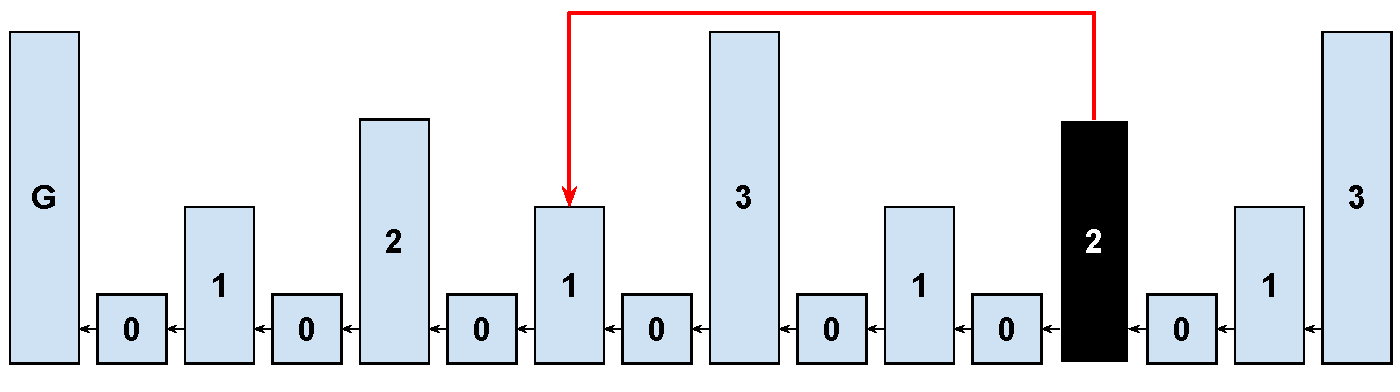
\includegraphics[width=0.7\columnwidth]{figures/simple_thorny.pdf}
    \caption{A thorny pointer of an adversarial block, colored black, in an honest party's chain. The thorny block points to a $1$-superblock which is an ancestor
		$1$-superblock, but not the \emph{most recent} ancestor $1$-superblock.}
	\label{fig:skip_ancestor}
\end{figure}

We conclude that the honest verifier comparing the honest superchain
against the adversarial superchain will reach the same conclusion in a velvet
fork as he would have reached in a soft fork: Because the honest
superchain in the velvet case contains the same amount of blocks as the honest
superchain in the soft fork case, but the adversarial superchain in the velvet
case contains fewer blocks than in the soft fork case, the comparison will
remain in favor of the honest party. As described in Section~\ref{sec:attack}, this
conclusion is incorrect.